%%%%%%%%%%%%%%%%%%%%%%%%%%%%%%%%%%%%%%%%%%%%%%%%%%%%%%%%%%%%
%%%%%%%%%%%%%%%%%%%%%%%%%%%%%%%%%%%%%%%%%%%%%%%%%%%%%%%%%%%%
%%%%%%%%%%%%%%%%%%%%%%%%%%%%%%%%%%%%%%%%%%%%%%%%%%%%%%%%%%%%
\section{The Dune Workflow for Simulations with CAD-Models}\label{Sec:Workflow}
%%%%%%%%%%%%%%%%%%%%%%%%%%%%%%%%%%%%%%%%%%%%%%%%%%%%%%%%%%%%
%%%%%%%%%%%%%%%%%%%%%%%%%%%%%%%%%%%%%%%%%%%%%%%%%%%%%%%%%%%%
%%%%%%%%%%%%%%%%%%%%%%%%%%%%%%%%%%%%%%%%%%%%%%%%%%%%%%%%%%%%

%-------------------------------------------------------------------
\subsection{Overview}
% Bilder
% Tool Chain

\begin{frame}
  \frametitle<presentation>{Overview}
  \begin{itemize}
    \item Real world problems have complex computational domains.
    \item One possibility to model such domains is CAD modelling.
    \item Need ability to import CAD models.
  \end{itemize}
  In Dune, the interface to CAD-Models is via \lstinline!Gmsh!.
\end{frame}

\begin{frame}
  \frametitle<presentation>{Some example meshes for CAD-meshes imported in Dune}
  \begin{figure}
    \begin{center}
      \includegraphics[width=0.48\textwidth]{./EPS/motor}  $\hspace{1mm}$
      \includegraphics[width=0.48\textwidth]{./EPS/shape2} $\hspace{1mm}$
      \caption[]{Some example meshes import to Dune.}
      \label{fig:CADExmapleMeshesToDune}
    \end{center}
  \end{figure}
\end{frame}

\begin{frame}
  \frametitle<presentation>{Overview}
  The outline to import meshed CAD-models in Dune is as follows
  \begin{itemize}
    \item Create or retrieve a CAD-model.
    \item Edit and mesh the CAD-model with Gmsh, a \ldots
    \item Export a \lstinline!.msh!-File from Gmsh.
    \item Import the mesh file with the \lstinline!Dune::GmshReader!.
  \end{itemize}
  We will show each step in detail in the following sections.
\end{frame}

%-------------------------------------------------------------------
\subsection{Gmsh and the DUNE Gmsh-Reader Interface}
% Dune GmshReader
% Gmsh und OpenCascade
% Installation
% welche Grids?

\begin{frame}[fragile]
  \frametitle{The Dune::GmshReader}
  We begin with the import of a Mesh file \lstinline!meshfile.msh! using Dune's
  \lstinline!GmshReader!:
  \begin{lstlisting}[basicstyle=\scriptsize]
// include gmshreader interface
#include<dune/grid/io/file/gmshreader.hh>
...
// construct grid from mesh file
Dune::UGGrid<2> grid(1000);
Dune::GmshReader<Dune::UGGrid<2> >::read(grid, "mesh.msh");
grid.globalRefine(3);
  \end{lstlisting}
  Note that you have to include the Gmsh-Interface header from
  \lstinline!dune-grid! to be able to import the meshes.
\end{frame}

\begin{frame}[fragile]
  \frametitle{Gmsh}
  The meshes are created and exported by Gmsh, an external Software,
  which is able to
  \begin{itemize}
    \item Import CAD models in various formats (\lstinline!GEO, STEP, IGES, BREP, ...!)
    \item Group subparts of the models into phyiscal \emph{entities} or
      \lstinline{groups},
    \item Mesh the models,
    \item Write the meshes including physical group regions to a mesh file
      (ending \lstinline!.msh!).
  \end{itemize}
\end{frame}

%\begin{frame}
%\frametitle{Example 1 Overview}
%The first example implements model problem \eqref{Eq:Example01}.
%
%It consists of the following files:
%\begin{itemize}
%\item \lstinline{example01.cc} -- the file to be compiled.
%\item \lstinline{example01_main.hh} -- main function. Instantiates a grid and runs the variants.
%\item \lstinline{example01a_Q1.hh} -- solve model problem \eqref{Eq:Example01} with $Q_1$ elements.
%\item \lstinline{example01a_Q2.hh} -- same with $Q_2$ elements.
%\item \lstinline{example01a_RT.hh} -- same with nonconforming rotated bilinear (``Rannacher-Turek'' element).
%\item \lstinline{example01a_operator.hh} -- local operator implementing $\bm{\alpha}_{h,e}^{\text{vol}}$.
%\item \lstinline{example01b_Q2.hh} -- solve nonlinear variant of the model problem \eqref{Eq:Example01} with $Q_2$ elements.
%\item \lstinline{example01b_operator.hh} -- the local operator for the nonlinear variant.
%\end{itemize}
%\end{frame}
%
%\begin{frame}<presentation>[fragile,allowframebreaks,allowdisplaybreaks]
%\frametitle<presentation>{Function \lstinline{main}}
%\framesubtitle<presentation>{File \texttt{examples/example01\_main.hh}}
%\lstinputlisting[basicstyle=\tiny,numbers=left,
%numberstyle=\tiny, numbersep=2pt]{../../examples/example01_main.hh}
%\end{frame}
%\mode<article>{
%For completeness we show the main function that just instantiates a \lstinline{YaspGrid} object
%and calls the variants.
%
%Main functions will not be shown in later examples.
%
%\begin{Lst}[File examples/example01\_main.hh] \mbox
%\nopagebreak
%\lstinputlisting[basicstyle=\scriptsize,numbers=left,
%numberstyle=\tiny, numbersep=2pt]{../../examples/example01_main.hh}
%\end{Lst}}
%
%
%\begin{frame}
%\frametitle{Driver for Solving Stationary Linear Problems}
%\framesubtitle{About \lstinline{example01a_Q1.hh}}
%\begin{enumerate}
%\item Define useful constants/types like dimension or basic numeric type.
%\item Make \textit{grid function space} which corresponds here to $U_h^k$. It requires
%\begin{itemize}
%\item a \textit{finite element map} defining a local basis on each element.
%\item a method to set up \textit{constraints} on the function space (empty here).
%\item a suitable vector backend.
%\end{itemize}
%\item Make \textit{grid operator space} computing $\mathcal{R}(\mathbf{u})$, $\nabla\mathcal{R}(\mathbf{u})$. It requires
%\begin{itemize}
%\item a local operator which provides $\bm{\alpha}_{h,e}^{\text{vol}}$.
%\item trial and test grid function spaces, possibly with constraints.
%\item a suitable matrix backend.
%\end{itemize}
%\item Select a linear solver backend (see vector/matrix backend).
%\item Solve the linear problem given with the selected solver backend.
%\begin{itemize}
%\item \textit{Vector container} is used to store degrees of freedom $\mathbf{u}\in\mathbf{U}$.
%\end{itemize}
%\item Output graphics files to visualize solution with ParaView.
%\begin{itemize}
%\item \textit{Discrete grid function} implements finite element isomorphism.
%\end{itemize}
%\end{enumerate}
%\end{frame}
%
%
%\begin{frame}<presentation>[fragile,allowframebreaks,allowdisplaybreaks]
%\frametitle<presentation>{Unconstrained Elliptic Problem with $Q_1$}
%\framesubtitle<presentation>{File \texttt{examples/example01a\_Q1.hh}}
%\lstinputlisting[basicstyle=\tiny,numbers=left,
%numberstyle=\tiny, numbersep=2pt]{../../examples/example01a_Q1.hh}
%\end{frame}
%\mode<article>{
%\begin{Lst}[File examples/example01a\_Q1.hh] \mbox
%\nopagebreak
%\lstinputlisting[basicstyle=\scriptsize,numbers=left,
%numberstyle=\tiny, numbersep=2pt]{../../examples/example01a_Q1.hh}
%\end{Lst}}
%
%
%\begin{frame}
%\frametitle{Local Operator}
%\begin{itemize}
%\item The local operator implements $\bm{\alpha}_{h,e}^{\text{vol}}$ (and more).
%\item Class template \lstinline{GridOperatorSpace} builds on a local operator and
%provides $\mathcal{R}(\mathbf{u})$, $\nabla\mathcal{R}(\mathbf{u})$ \textit{generically}.
%\item Works for many different discretizations (see below).
%\item Works as well for systems of PDEs (see below).
%\end{itemize}
%\end{frame}
%
%\begin{frame}
%\frametitle{Local Operator Implementation}
%\framesubtitle{About \lstinline{example01a_operator.hh}}
%A local operator is a class providing the following:
%\begin{itemize}
%\item Flags controlling the sparsity pattern assembly.
%\item Method \lstinline{pattern_volume} assembling sparsity pattern (default provided).
%\item Flags controlling which terms to assemble.
%\item Method \lstinline{alpha_volume} computing $\bm{\alpha}_{h,e}^{\text{vol}}(\mathbf{u})$.
%\item Method \lstinline{jacobian_volume} computing $\nabla\bm{\alpha}_{h,e}^{\text{vol}}(\mathbf{u})$.
%This method can be provided generically through numerical differentiation.
%\item Method \lstinline{jacobian_apply_volume} computing $\nabla\bm{\alpha}_{h,e}^{\text{vol}}(\mathbf{u})\mathbf{u}$.
%This method can be provided generically through numerical differentiation.
%\item Possibly more methods (to be introduced later):
%\begin{itemize}
%\item \lstinline{alpha_boundary}, \lstinline{alpha_skeleton} -- boundary/interior face integrals.
%\item \lstinline{lambda_volume}, \lstinline{lambda_boundary} -- parts of the residual depending on the test function only (optional).
%\end{itemize}
%\end{itemize}
%\end{frame}
%
%\begin{frame}[fragile]
%\frametitle{\lstinline{alpha_volume} Method}
%The method \lstinline{alpha_volume} has the following signature:
%\begin{lstlisting}[basicstyle=\scriptsize]
%template<typename EG, typename LFSU, typename X,
%         typename LFSV, typename R>
%void alpha_volume (const EG& eg, const LFSU& lfsu, const X& x,
%                   const LFSV& lfsv, R& r) const;
%\end{lstlisting}
%Where the arguments are:
%\begin{itemize}
%\item \lstinline{eg} -- a codim 0 entity $e\in E_h^0$.
%\item \lstinline{lfsu} -- local basis $\hat\phi_{e,l}$ for trial space.
%\item \lstinline{x} -- local coefficients $(\mathbf{u})_l$.
%\item \lstinline{lfsv} -- local basis $\hat\psi_{e,l}$ for the test space
%\item \lstinline{r} -- local contribution to residual (the result).
%\end{itemize}
%\end{frame}
%
%
%\begin{frame}<presentation>[fragile,allowframebreaks,allowdisplaybreaks]
%\frametitle<presentation>{Local Operator for Unconstrained Elliptic Problem}
%\framesubtitle<presentation>{File \texttt{examples/example01a\_operator.hh}}
%\lstinputlisting[basicstyle=\tiny,numbers=left,
%numberstyle=\tiny, numbersep=2pt]{../../examples/example01a_operator.hh}
%\end{frame}
%\mode<article>{
%\begin{Lst}[File examples/example01a\_operator.hh] \mbox
%\nopagebreak
%\lstinputlisting[basicstyle=\scriptsize,numbers=left,
%numberstyle=\tiny, numbersep=2pt]{../../examples/example01a_operator.hh}
%\end{Lst}}
%
%\begin{frame}<presentation>
%\frametitle{Visualization of Example 1 Results}
%Left figure shows the results for $Q_1$ elements.
%
%But we can do easily other elements as well \ldots
%
%\begin{center}
%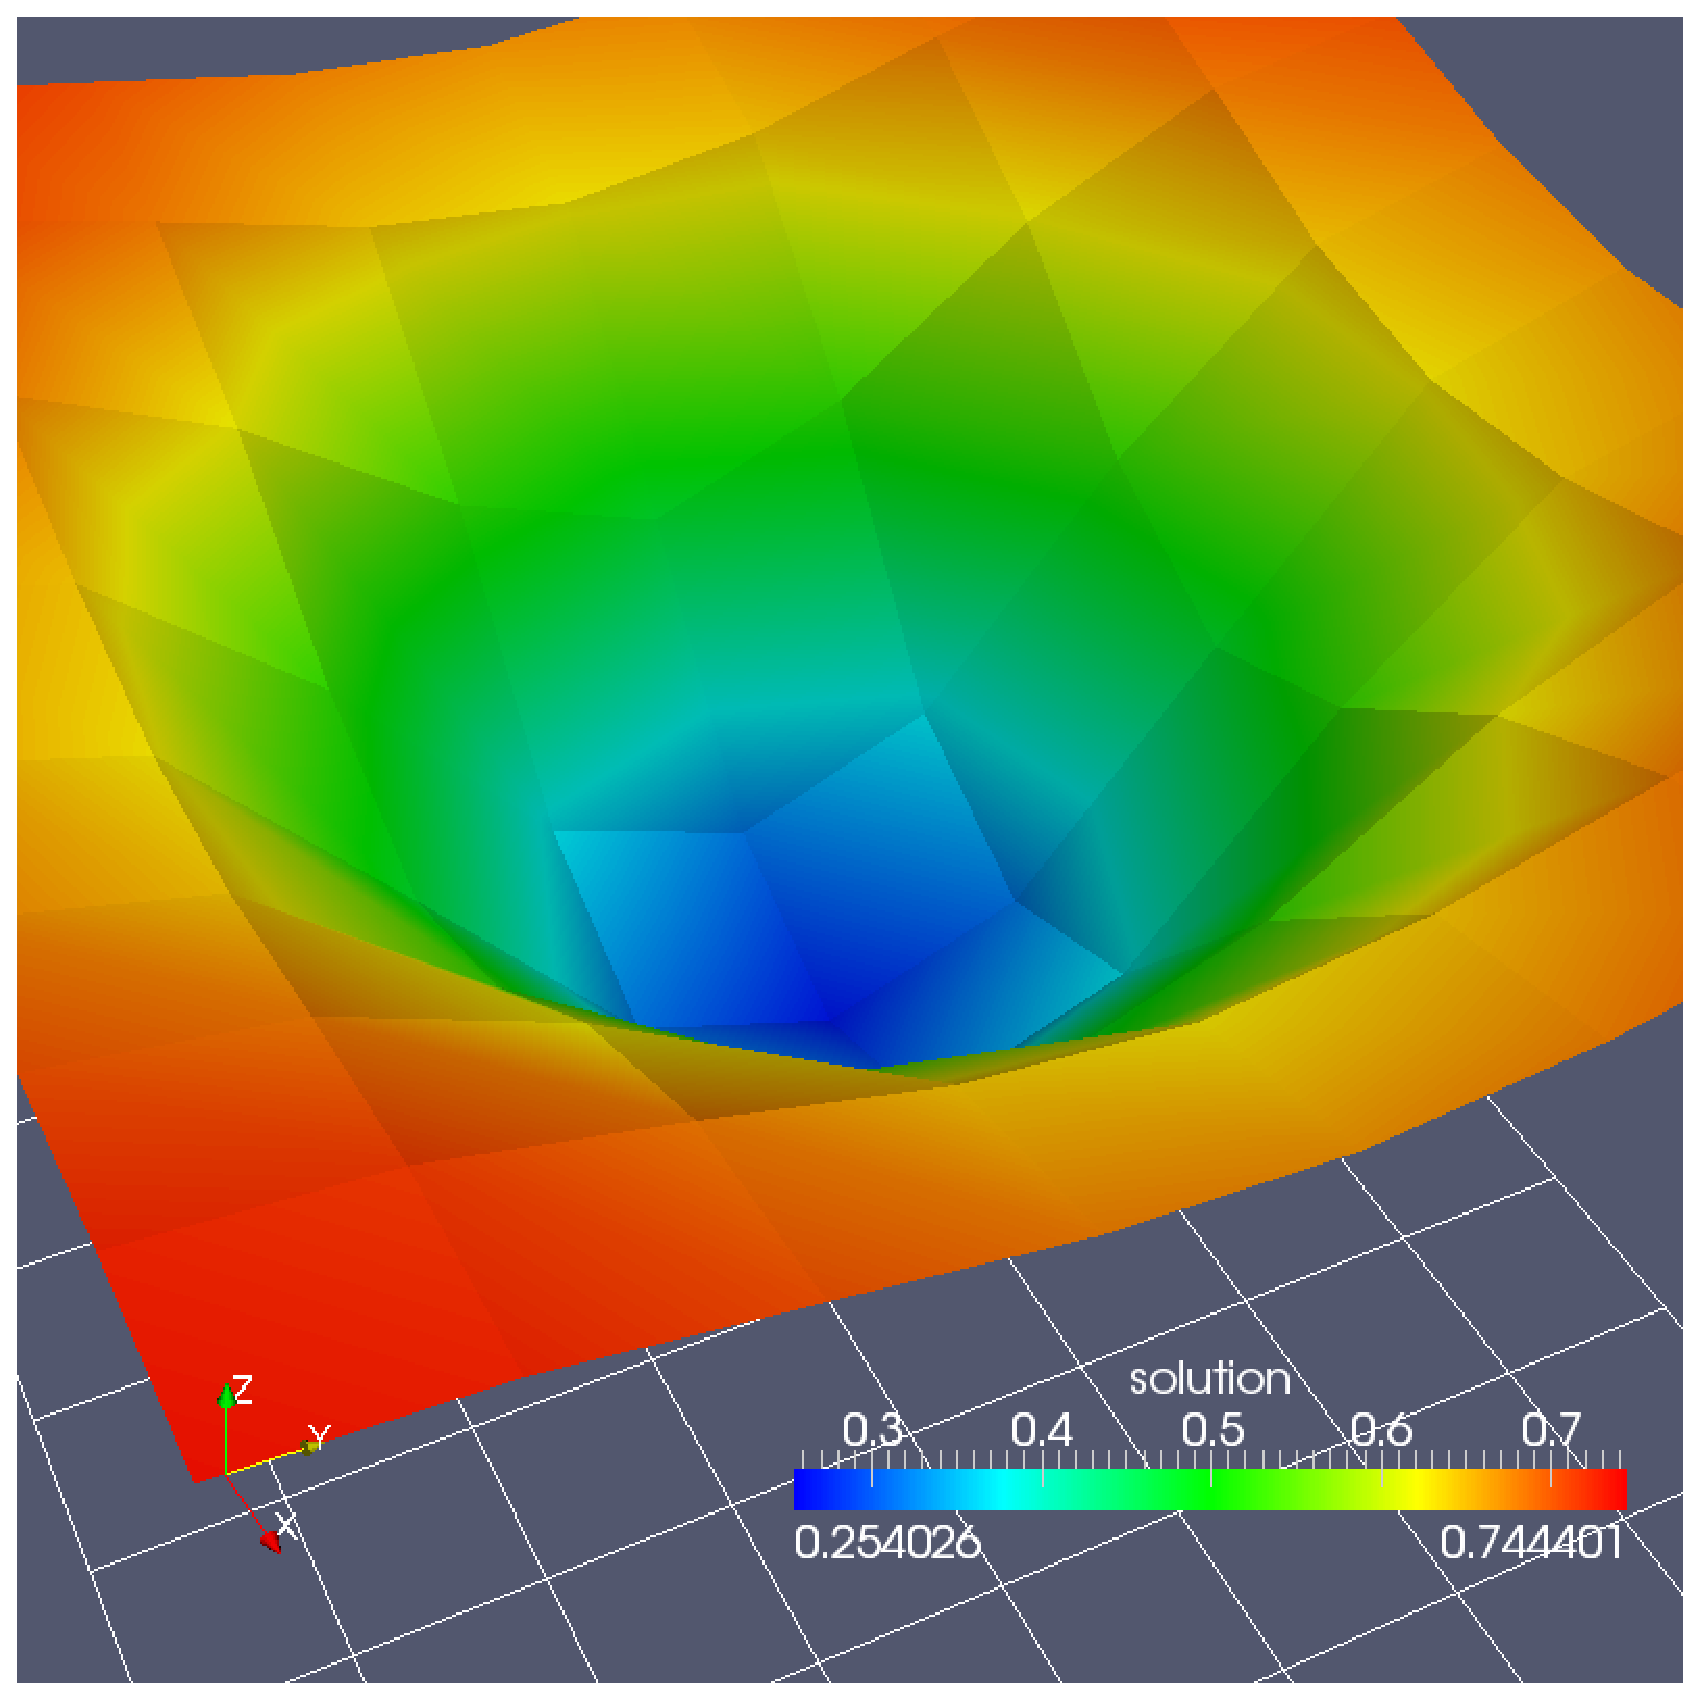
\includegraphics[width=0.32\textwidth]{./EPS/example01a_Q1} $\hspace{1mm}$
%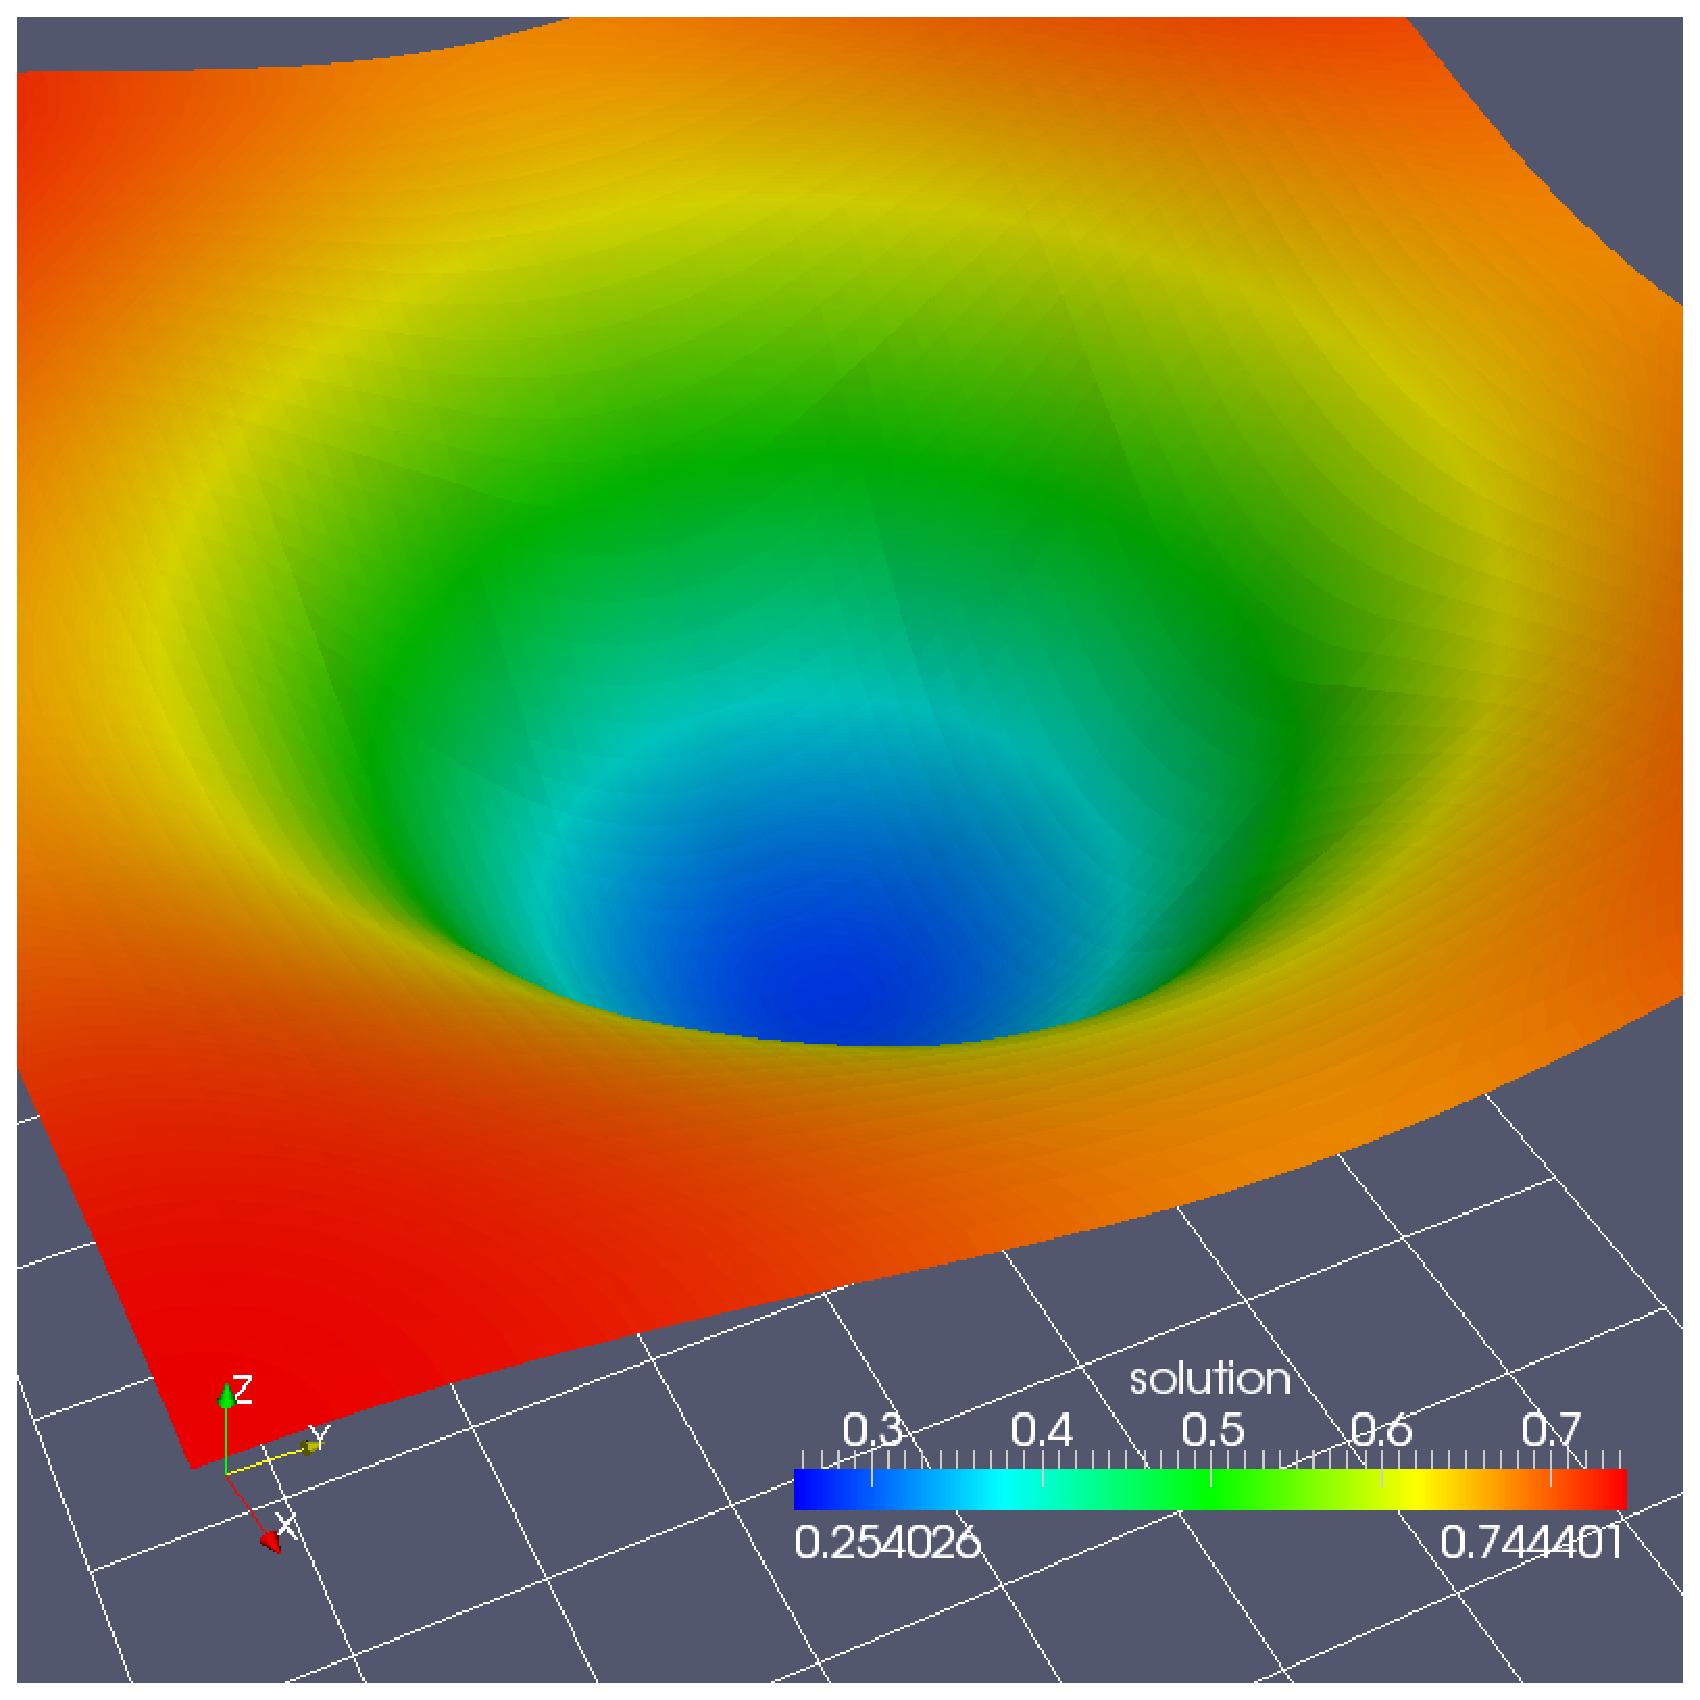
\includegraphics[width=0.32\textwidth]{./EPS/example01a_Q2} $\hspace{1mm}$
%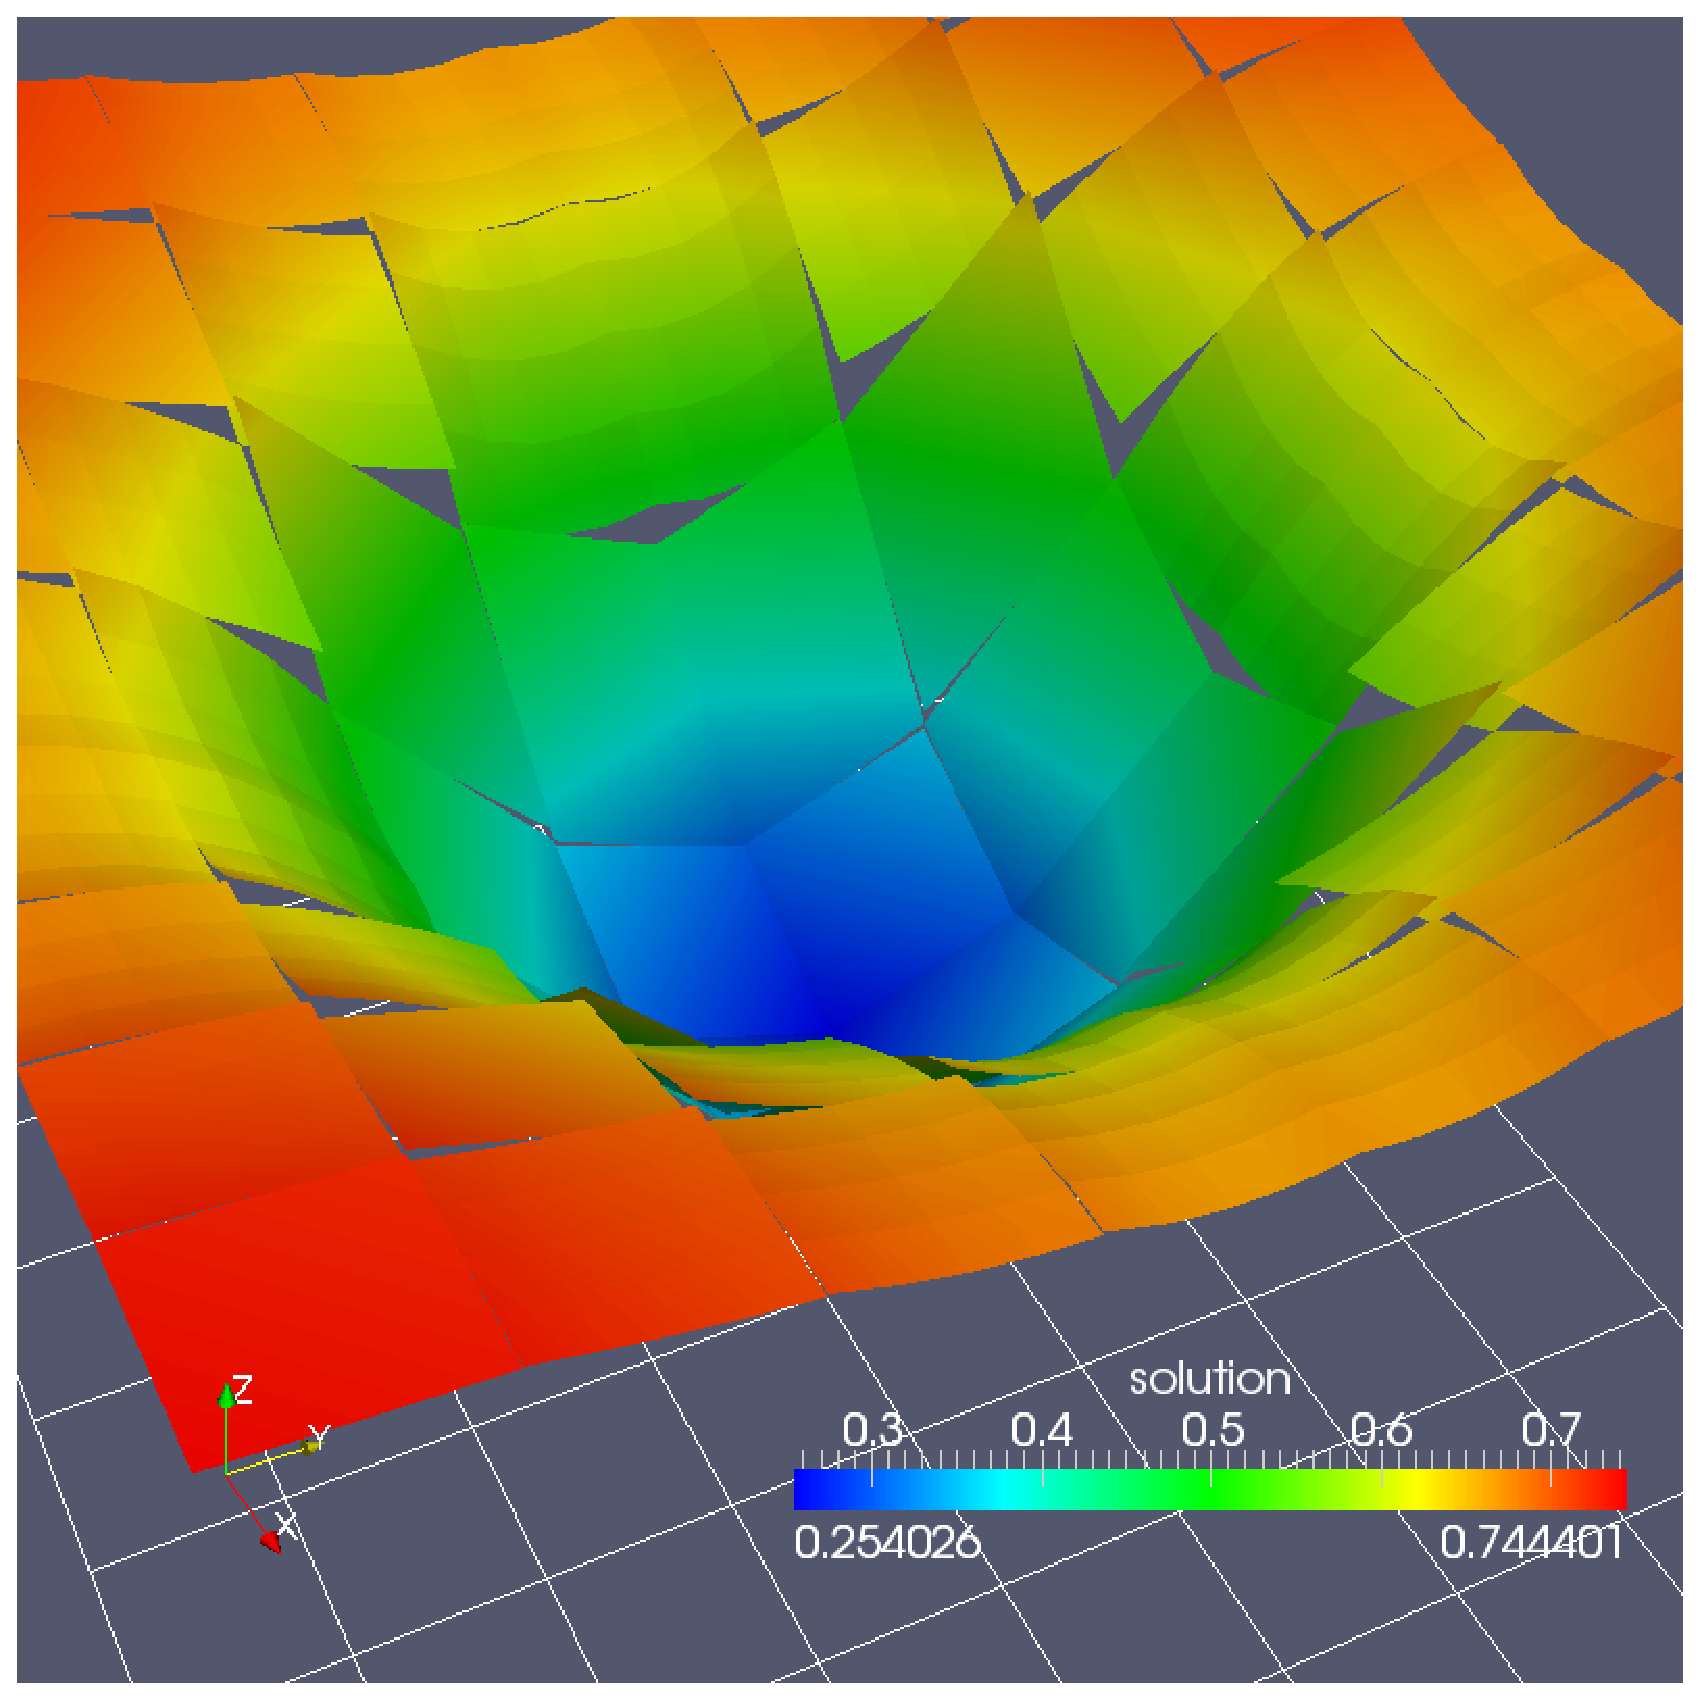
\includegraphics[width=0.32\textwidth]{./EPS/example01a_RT}
%
%$Q_1$ \hspace{30mm} $Q_2$ \hspace{30mm} $RT$
%\end{center}
%
%\mode<presentation>{
%More on that in the excercises!
%}
%\end{frame}
%
%\mode<article>{
%Figure \ref{fig:Example01aResults} shows visualizations of the results computed
%with \lstinline{example01}.
%\begin{figure}
%\begin{center}
%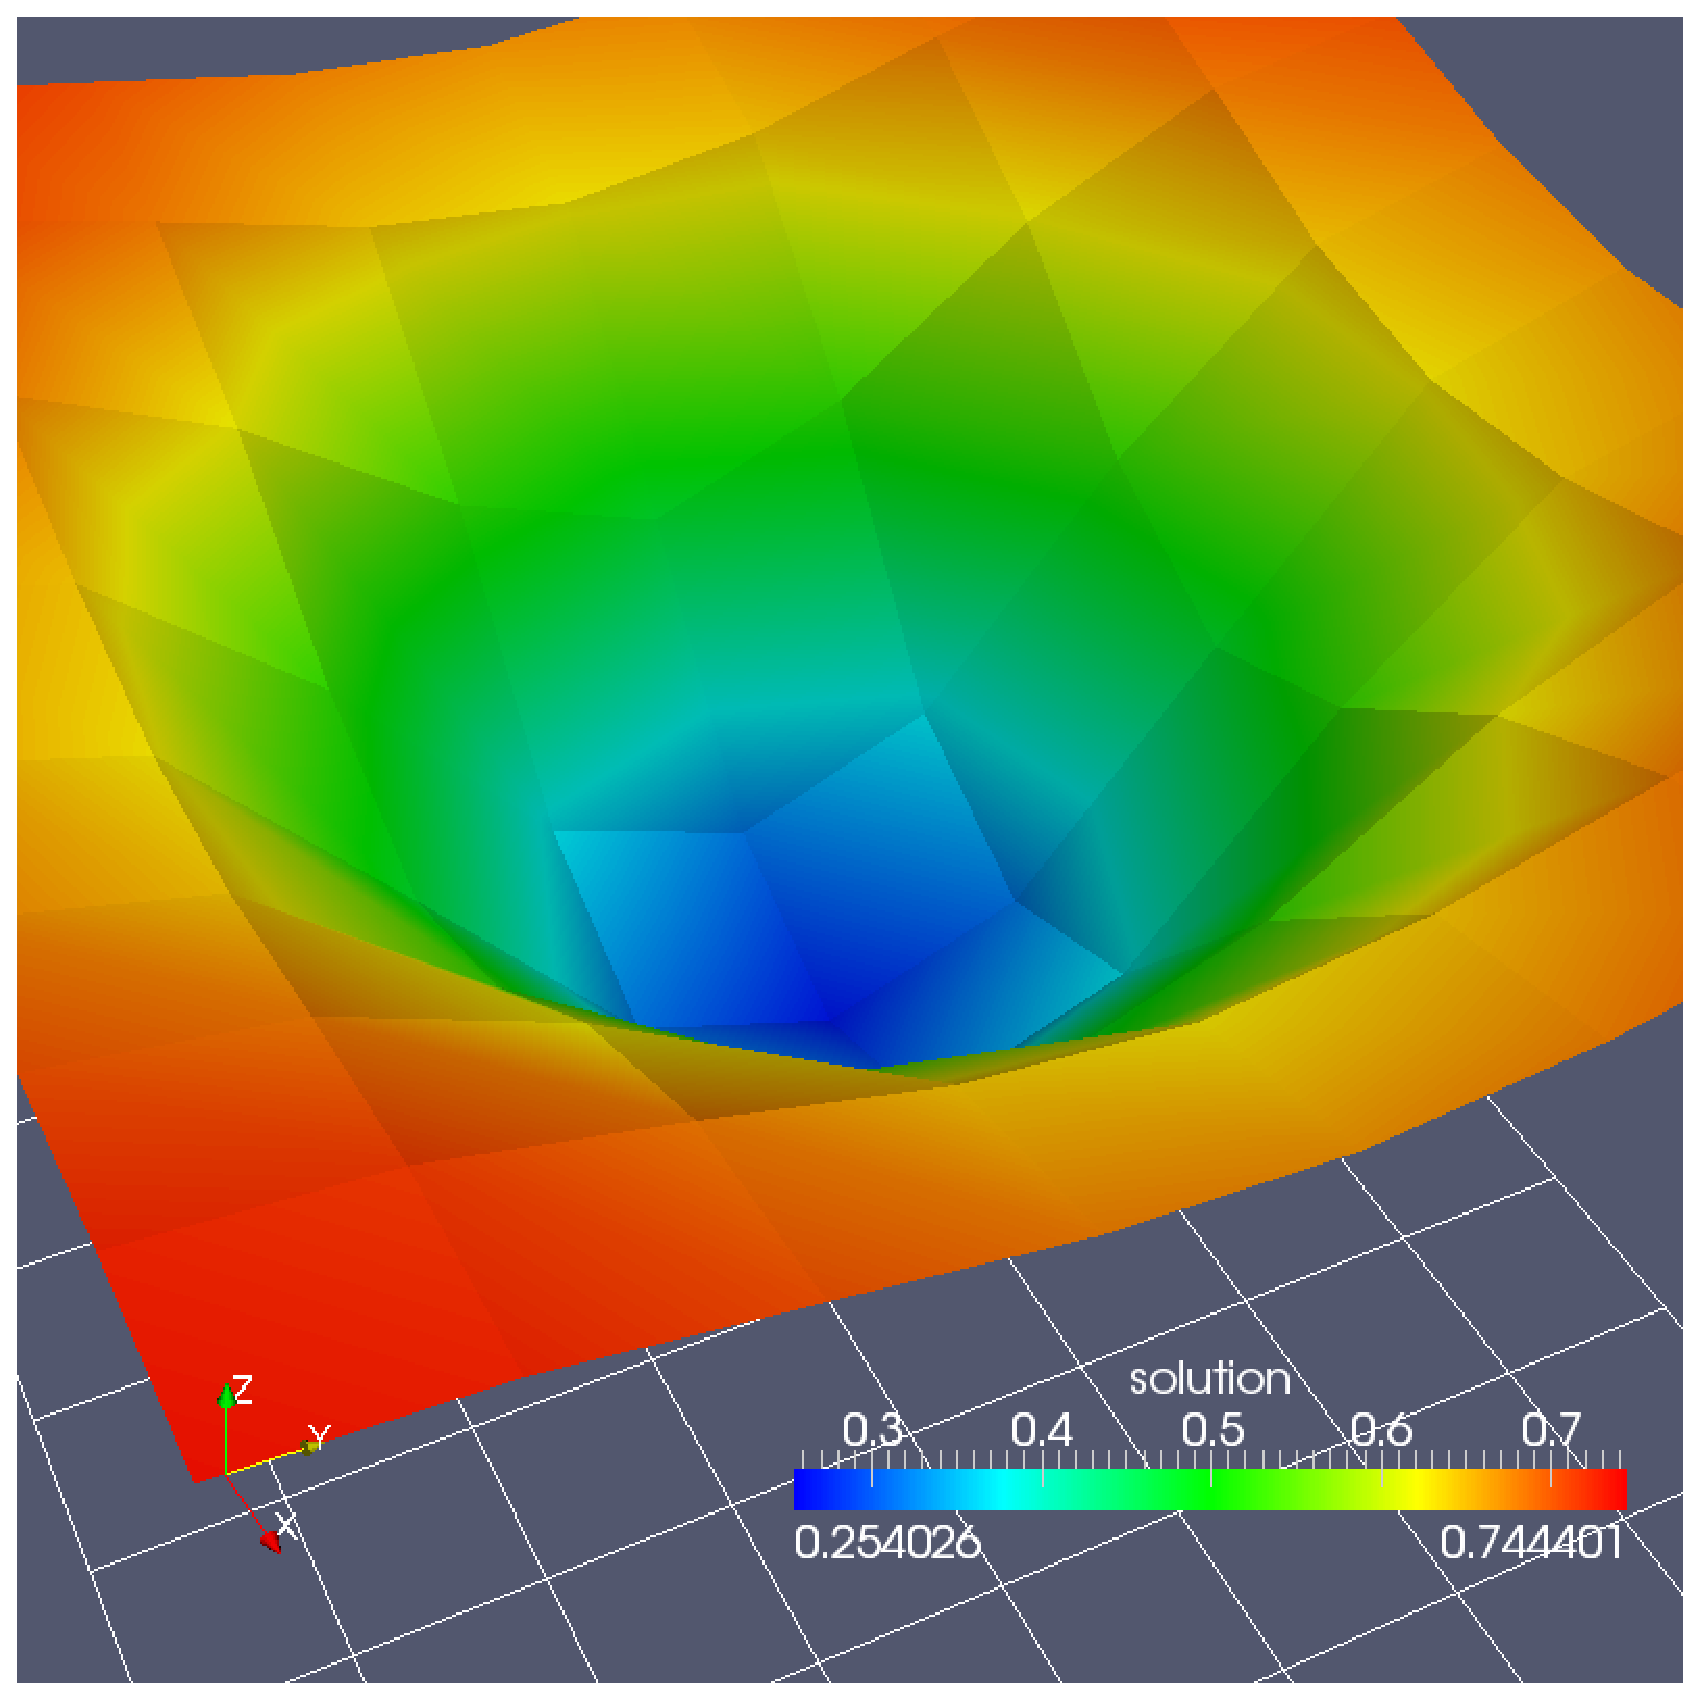
\includegraphics[width=0.32\textwidth]{./EPS/example01a_Q1} $\hspace{1mm}$
%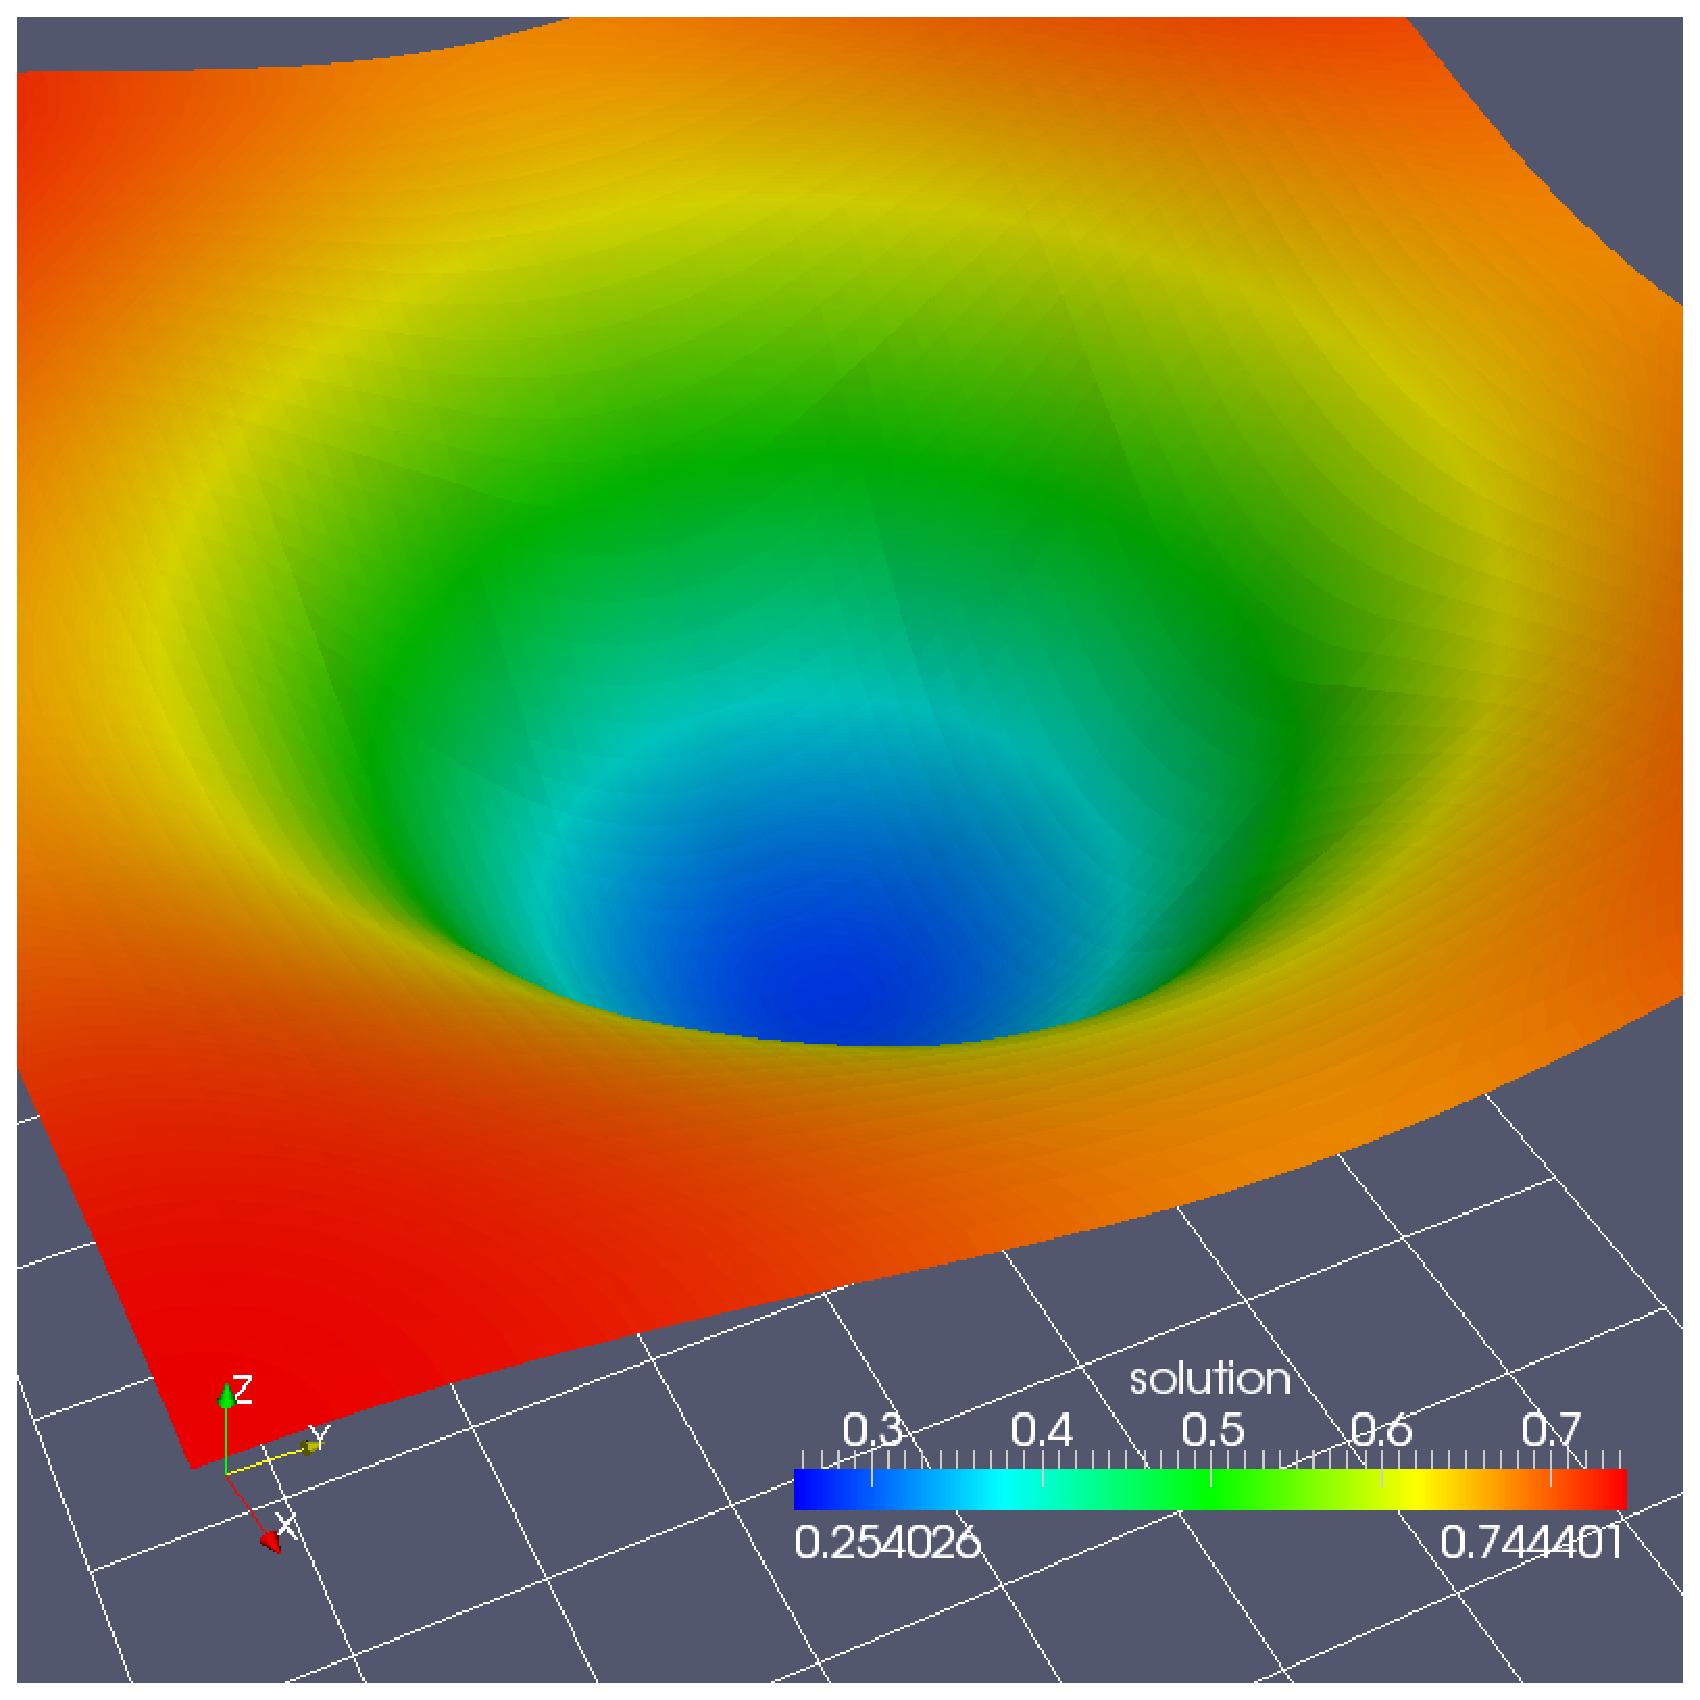
\includegraphics[width=0.32\textwidth]{./EPS/example01a_Q2} $\hspace{1mm}$
%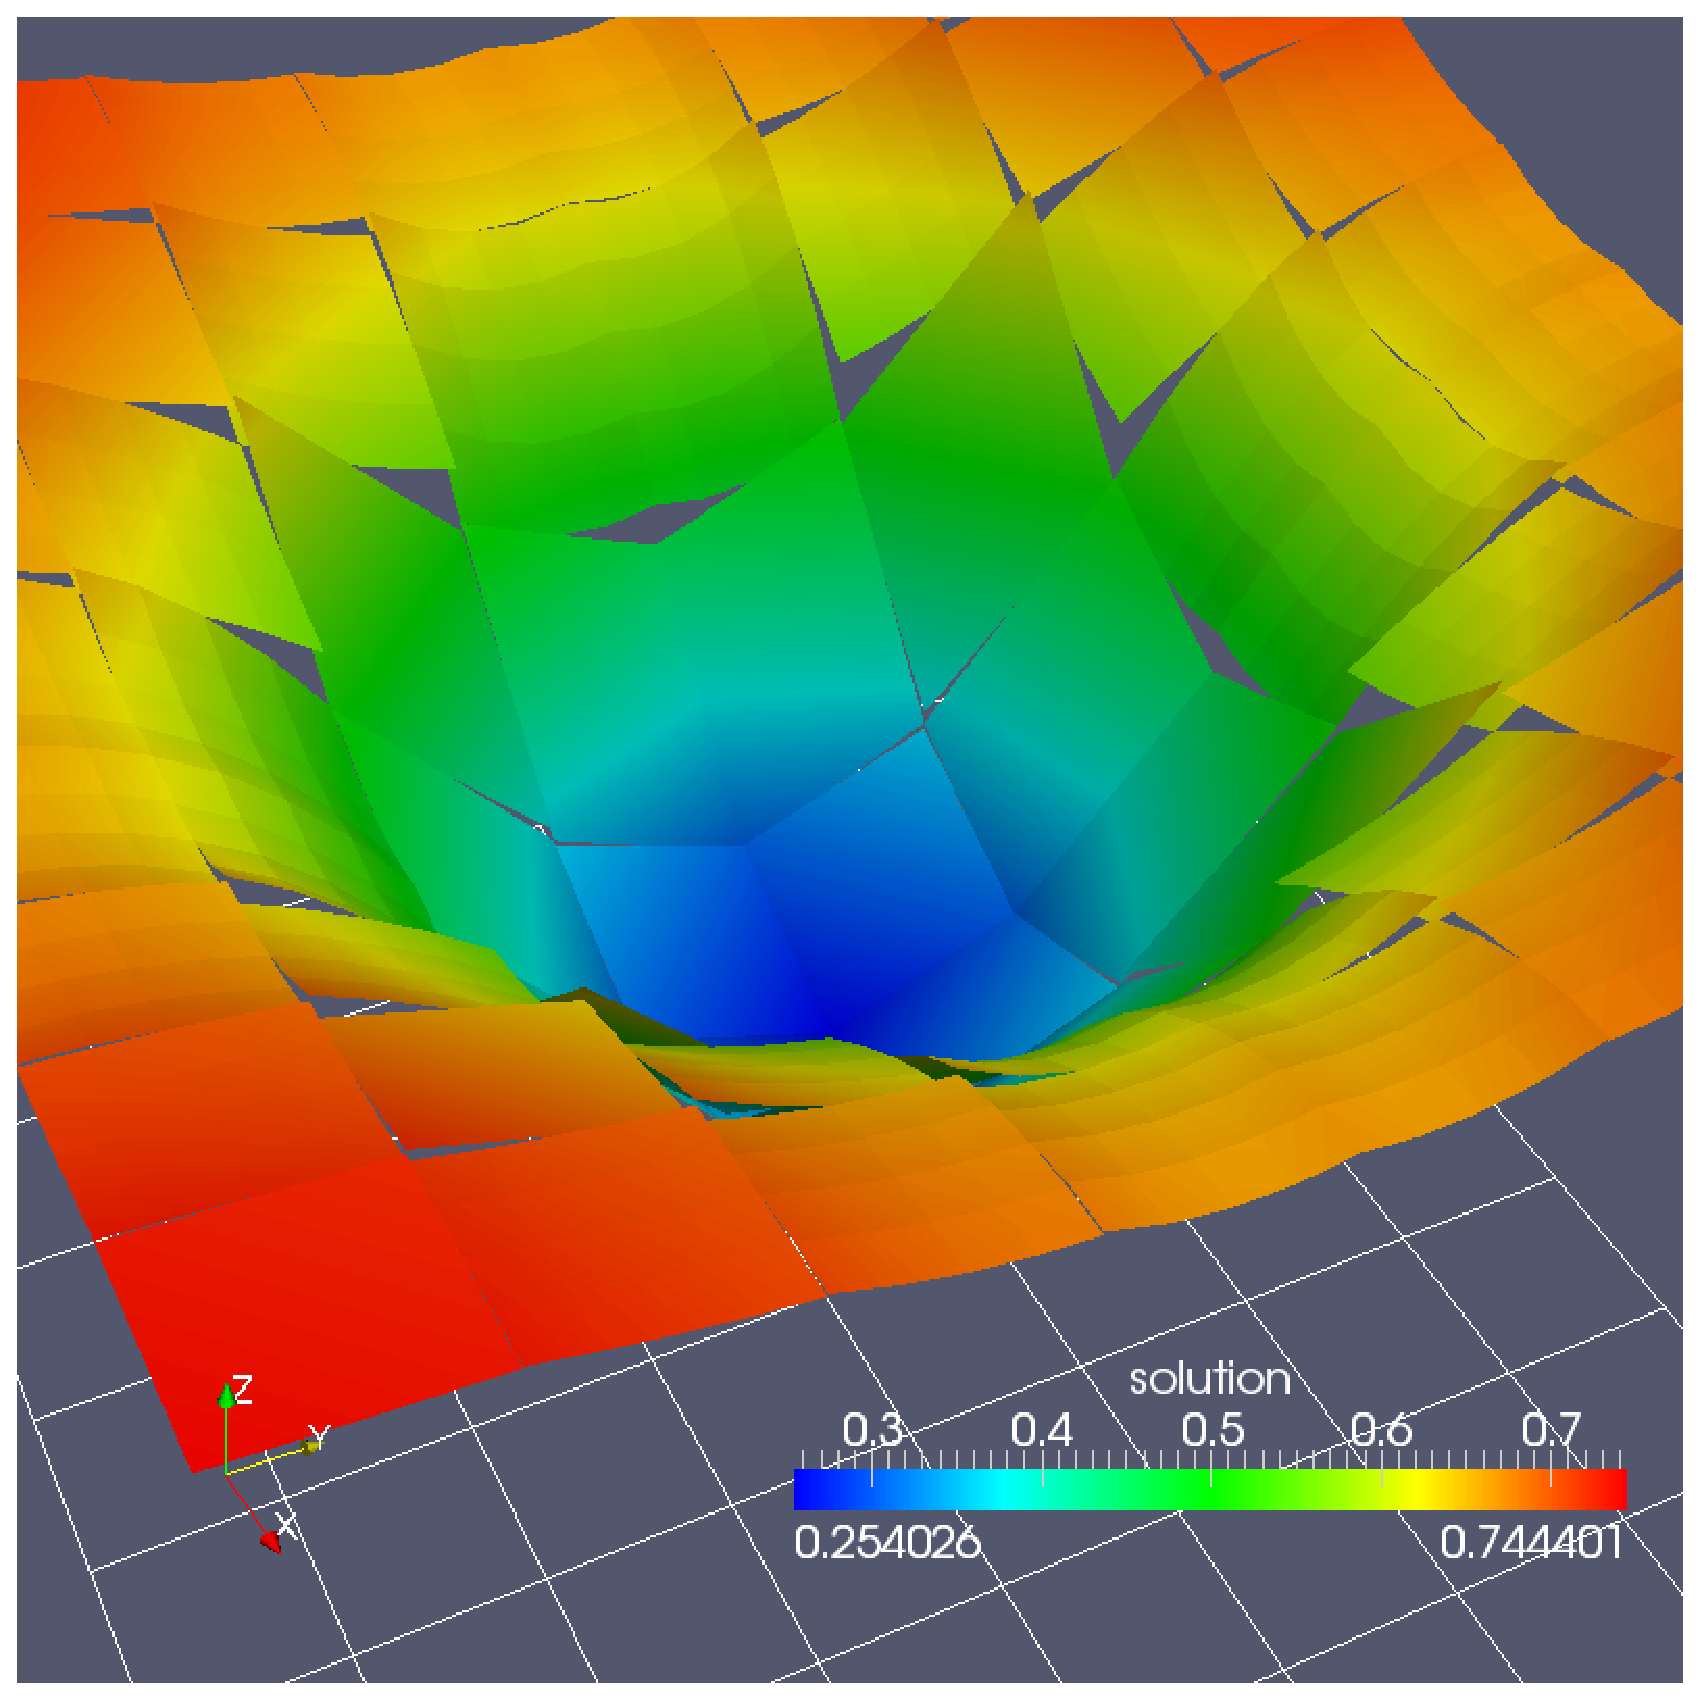
\includegraphics[width=0.32\textwidth]{./EPS/example01a_RT}
%\end{center}
%\caption{Results for example 1a computed with three different finite element spaces.
%From left: $Q_1$ elements, $Q_2$ elements, rotated bilinear (Rannacher-Turek)
%element on an $8 \times 8$ grid.}
%\label{fig:Example01aResults}
%\end{figure}
%}
%
%
%\begin{frame}
%\frametitle{Using $Q_2$ Elements}
%\ldots is quite simple, see \lstinline{example01a_Q2.hh}. Just
%\begin{itemize}
%\item Use another finite element map \lstinline{Q22DLocalFiniteElementMap}.
%\item Increase quadrature order on the local operator to 4.
%\item Use \lstinline{SubsamplingVTKWriter} to allow visualization of higher order polynomials.
%\item Use a new name for the output file.
%\end{itemize}
%
%Explore the Rannacher Turek element in \lstinline{example01a_RT.hh}
%\end{frame}
%
%
%\begin{frame}<presentation>[fragile,allowframebreaks,allowdisplaybreaks]
%\frametitle<presentation>{Unconstrained Elliptic Problem with $Q_2$}
%\framesubtitle<presentation>{File \texttt{examples/example01a\_Q2.hh}}
%\lstinputlisting[basicstyle=\tiny,numbers=left,
%numberstyle=\tiny, numbersep=2pt]{../../examples/example01a_Q2.hh}
%\end{frame}
%\mode<article>{
%\begin{Lst}[File examples/example01a\_Q2.hh] \mbox
%\nopagebreak
%\lstinputlisting[basicstyle=\scriptsize,numbers=left,
%numberstyle=\tiny, numbersep=2pt]{../../examples/example01a_Q2.hh}
%\end{Lst}}
%
%
%\begin{frame}
%\frametitle{Going Nonlinear}
%\ldots is also easy. Just
%\begin{itemize}
%\item Make a new local operator where the coefficients $a$ and $f$ depend on the solution $u$,
%see \lstinline{example01b_operator}.
%\item Use this new local operator in the grid operator space.
%\item Use class \lstinline{Newton} to solve the nonlinear algebraic problem.
%\item Use a new name for the output file :-).
%\end{itemize}
%\end{frame}
%
%\begin{frame}<presentation>[fragile,allowframebreaks,allowdisplaybreaks]
%\frametitle<presentation>{Unconstrained Nonlinear Elliptic Problem with $Q_2$}
%\framesubtitle<presentation>{File \texttt{examples/example01b\_Q2.hh}}
%\lstinputlisting[basicstyle=\tiny,numbers=left,
%numberstyle=\tiny, numbersep=2pt]{../../examples/example01b_Q2.hh}
%\end{frame}
%\mode<article>{
%\begin{Lst}[File examples/example01b\_Q2.hh] \mbox
%\nopagebreak
%\lstinputlisting[basicstyle=\scriptsize,numbers=left,
%numberstyle=\tiny, numbersep=2pt]{../../examples/example01b_Q2.hh}
%\end{Lst}}


%-------------------------------------------------------------------
\subsection{Importing and Meshing CAD-Geometries with Gmsh}
% CAD-Files Uebersicht
% install with opencascade
% Import
% Welcher Mesher?

\begin{frame}
  \frametitle{Common CAD-File formats}
  \begin{table}
    Amongst the most common CAD-File formats are
    \begin{center}
      \begin{tabular}{|c|c|c|}
        \hline
        Format & Ending & Description
        \\
        \hline
        STEP & \lstinline!.stp! &
        \\
        \hline
        BREP & \lstinline!.brp! &
        \\
        \hline
        IGES & \lstinline!.igs, .iges! &
        \\
        \hline
        GEO & \lstinline!.geo! & Native Gmsh format
        \\
        \hline
      \end{tabular}
      \caption{Some CAD file formats.}
      \label{tab:CADFileFormats}
    \end{center}
  \end{table}
\end{frame}

%\begin{frame}
%\frametitle{What is different ?}
%\begin{itemize}
%\item The residual form has a new term which is a boundary integral.
%\begin{itemize}
%\item There will be an additional method on the local operator.
%\end{itemize}
%\item The problem is solved in an affine subspace.
%We call $\tilde{U}$ a \textit{constrained space}.
%\item In the linear case it suffices to solve a problem with homogeneous Dirichlet
%boundary conditions:
%\begin{subequations}
%\begin{align*}
% -\Delta \bar{u} + a \bar{u}  &= f + \Delta w - a w &&\text{in $\Omega\subset\mathbb{R}^d$},\\
%                \bar{u} &= 0 &&\text{on $\Gamma_D\subseteq\partial\Omega$},\\
%-\nabla \bar{u} \cdot n &= j+\nabla w\cdot n &&\text{on $\Gamma_N=\partial\Omega\setminus\Gamma_D$},
%\end{align*}
%where $w$ is an extension of $g$ to $\Omega$ and $u = w + \bar{u}$.
%\end{subequations}
%\item In the nonlinear case this is not possible.
%\end{itemize}
%\end{frame}
%
%
%\begin{frame}
%\frametitle{Finite Element Spaces in Constrained Case}
%\begin{itemize}
%\item Define appropriate finite-dimensional subspace:
%\begin{equation*}
%\tilde{U}_h^k = \left \{ u \in U_h^k \,:\, u|_{\Gamma_D} = 0 \right\} \subset U_h^k.
%\end{equation*}
%(Mesh resolves the Dirichlet bopundary $\Gamma_D$.
%\item Provide extension $w\in U_h^k$ with ``$w=g$'' on $\Gamma_D$ in an appropriate sense.
%\item Obviously, $\text{dim}\tilde{U}_h^k < \text{dim} U_h^k$.
%\item Note: Dirichlet boundary conditions could also be handled by penalty methods.
%This can be done easily in PDELab but is not shown here.
%\end{itemize}
%\end{frame}
%
%\begin{frame}
%\frametitle{General Constrained Spaces}
%\begin{itemize}
%\item Constrained spaces turn up in a number of other cases:
%\begin{itemize}
%\item Hanging nodes.
%\item Functions with zero average, rigid body modes.
%\item Varying polynomial degree in conforming finite elements ($p$-method).
%\item Periodic boundary conditions.
%\item Artificial essential boundary conditions or ghost degrees of freedom in parallelization.
%\end{itemize}
%\item PDELab has a general concept to handle all types of constraints.
%\item Given $U_h$ with index set $\mathcal{I}_{U_h^k}$, construct a basis of the subspace:
%\begin{itemize}
%\item Partition index set: $\mathcal{I}_{U_h^k} = \tilde{\mathcal{I}} \cup \bar{\mathcal{I}}$.
%\item Construct new basis from given basis:
%\begin{equation*}
%\tilde\phi_i = \phi_i + \sum\limits_{j\in\bar{\mathcal{I}}} \omega_{i,j} \phi_j, \qquad i\in\tilde{\mathcal{I}}.
%\end{equation*}
%\item $\tilde{U}_h$ is spanned by the new basis.
%\end{itemize}
%\item Constrained space defined by splitting $\tilde{\mathcal{I}} \cup \bar{\mathcal{I}}$
%and coefficients $\omega_{i,j}$.
%\end{itemize}
%\end{frame}


%-------------------------------------------------------------------
\subsection{Attaching Data to a CAD-Geometry and its Mesh}
% Gruppen in Gmsh
% Gmshreader nur eine Gruppe pro Element!
% PDELab-Code

\begin{frame}
  \frametitle<presentation>{Abstraction}
  Most simulations include parameters associated to some part of the
  domain, for instance
  \begin{itemize}
    \item Material properties (conductivities,\ldots),
    \item Variing boundary conditions,
    \item \ldots
  \end{itemize}
  Thus we need an ability to specify subdomains for our CAD-model.
  In Gmsh: \emph{Physical Groups}:
  \begin{itemize}
    \item Volume groups,
    \item Surface groups,
    \item Line groups.
    \item Point groups.
  \end{itemize}
\end{frame}

\begin{frame}
  \frametitle<presentation>{Abstraction}
  \begin{figure}
    \begin{center}
      \includegraphics[width=0.8\textwidth]{./EPS/crank/geo2} $\hspace{1mm}$
      \caption[]{Physical groups for a CAD-Model in Gmsh.}
      \label{fig:gmshPhysGroups}
    \end{center}
  \end{figure}
\end{frame}

\begin{frame}
  \frametitle<presentation>{Abstraction}
  The \lstinline!Dune::GmshReader! is able to read
  \begin{itemize}
    \item Volume groups, and
    \item Surface groups
  \end{itemize}
  from a \lstinline!.msh!-file. The following code shows that:
\end{frame}

%\begin{frame}<presentation>[fragile,allowframebreaks,allowdisplaybreaks]
%\frametitle<presentation>{Boundary Condition Type Function}
%\framesubtitle<presentation>{File \texttt{examples/example02\_bctype.hh}}
%\lstinputlisting[basicstyle=\tiny,numbers=left,
%numberstyle=\tiny, numbersep=2pt]{../../examples/example02_bctype.hh}
%\end{frame}
%\mode<article>{
%\begin{Lst}[File examples/example02\_bctype.hh] \mbox
%\nopagebreak
%\lstinputlisting[basicstyle=\scriptsize,numbers=left,
%numberstyle=\tiny, numbersep=2pt]{../../examples/example02_bctype.hh}
%\end{Lst}}
%
%\begin{frame}<presentation>[fragile,allowframebreaks,allowdisplaybreaks]
%\frametitle<presentation>{Boundary Condition Extension Function}
%\framesubtitle<presentation>{File \texttt{examples/example02\_bcextension.hh}}
%\lstinputlisting[basicstyle=\tiny,numbers=left,
%numberstyle=\tiny, numbersep=2pt]{../../examples/example02_bcextension.hh}
%\end{frame}
%\mode<article>{
%\begin{Lst}[File examples/example02\_bcextension.hh] \mbox
%\nopagebreak
%\lstinputlisting[basicstyle=\scriptsize,numbers=left,
%numberstyle=\tiny, numbersep=2pt]{../../examples/example02_bcextension.hh}
%\end{Lst}}
%
%\begin{frame}[fragile]
%\frametitle{\lstinline{alpha_boundary} Method}
%Local operator is extended by a new method \lstinline{alpha_boundary}
%computing the boundary integral.
%
%\lstinline{alpha_boundary} has the following signature:
%\begin{lstlisting}[basicstyle=\scriptsize]
%template<typename IG, typename LFSU, typename X,
%         typename LFSV, typename R>
%void alpha_boundary (const IG& ig, const LFSU& lfsu_s, const X& x_s,
%                     const LFSV& lfsv_s, R& r_s) const
%\end{lstlisting}
%Where the arguments are:
%\begin{itemize}
%\item \lstinline{ig} -- intersection with domain boundary.
%\item \lstinline{lfsu_s} -- local basis $\hat\phi_{e,l}$ for trial space on inside element.
%\item \lstinline{x_s} -- local coefficients on inside element.
%\item \lstinline{lfsv_s} -- local basis $\hat\psi_{e,l}$ for test space on inside element.
%\item \lstinline{r_s} -- local contribution to residual on inside element.
%\end{itemize}
%\end{frame}
%
%
%\begin{frame}<presentation>[fragile,allowframebreaks,allowdisplaybreaks]
%\frametitle<presentation>{Local Operator with Neumann Boundary}
%\framesubtitle<presentation>{File \texttt{examples/example02\_operator.hh}}
%\lstinputlisting[basicstyle=\tiny,numbers=left,
%numberstyle=\tiny, numbersep=2pt]{../../examples/example02_operator.hh}
%\end{frame}
%\mode<article>{
%\begin{Lst}[File examples/example02\_operator.hh] \mbox
%\nopagebreak
%\lstinputlisting[basicstyle=\scriptsize,numbers=left,
%numberstyle=\tiny, numbersep=2pt]{../../examples/example02_operator.hh}
%\end{Lst}}
%
%\begin{frame}<presentation>
%\frametitle{Visualization of Constrained Problem Results}
%Neumann boundary condition at $x=1$, Dirichlet elsewhere.
%
%\begin{center}
%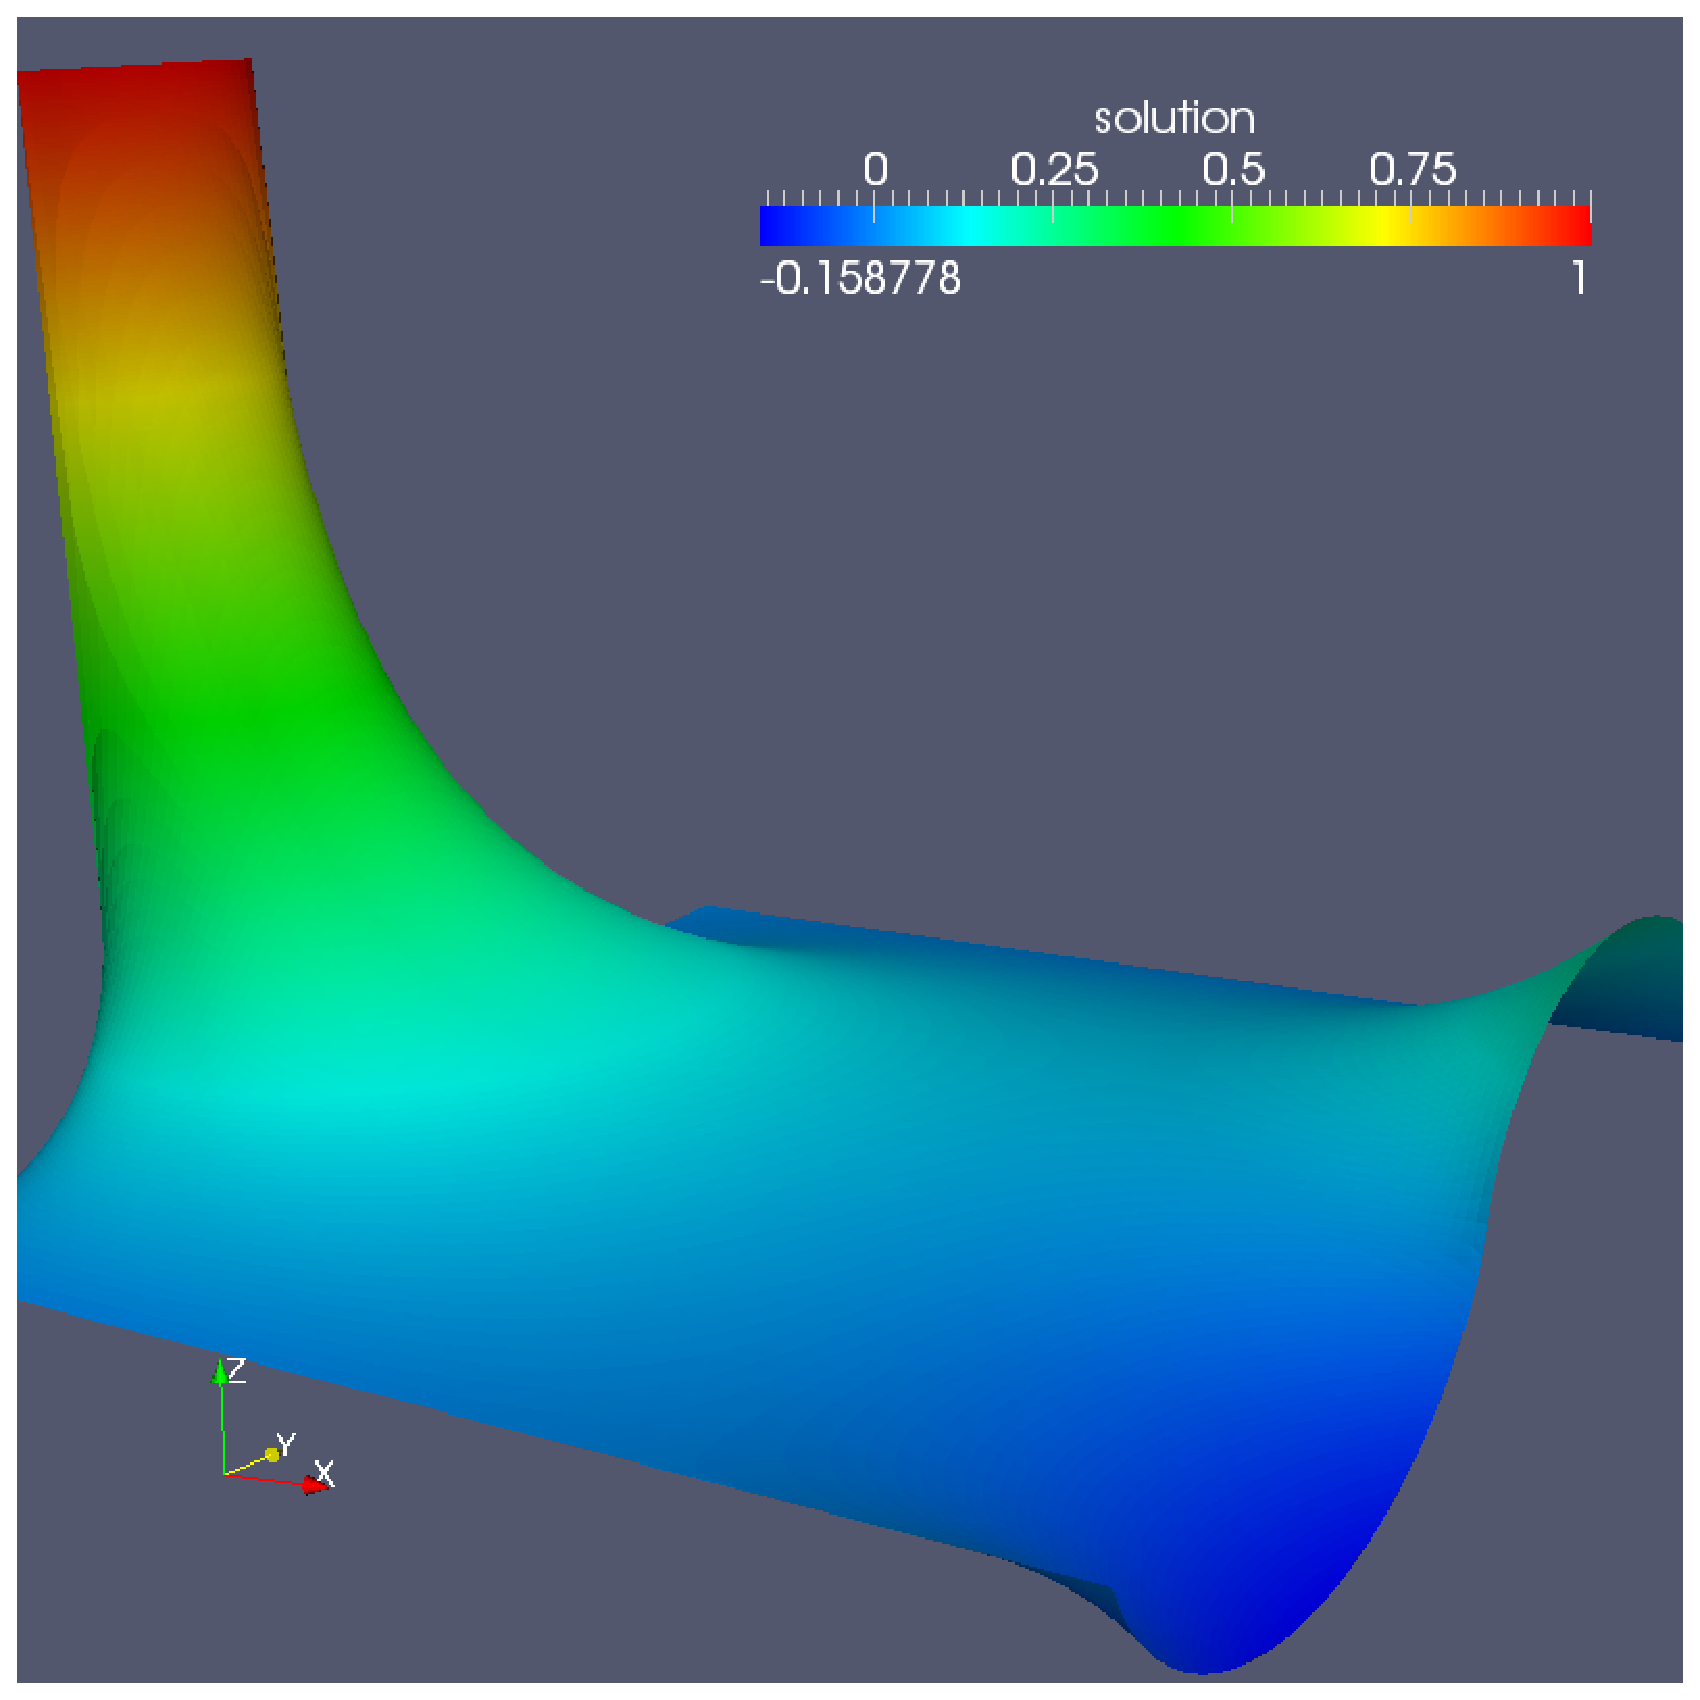
\includegraphics[width=0.48\textwidth]{./EPS/example02_Q1} \hspace{1mm}
%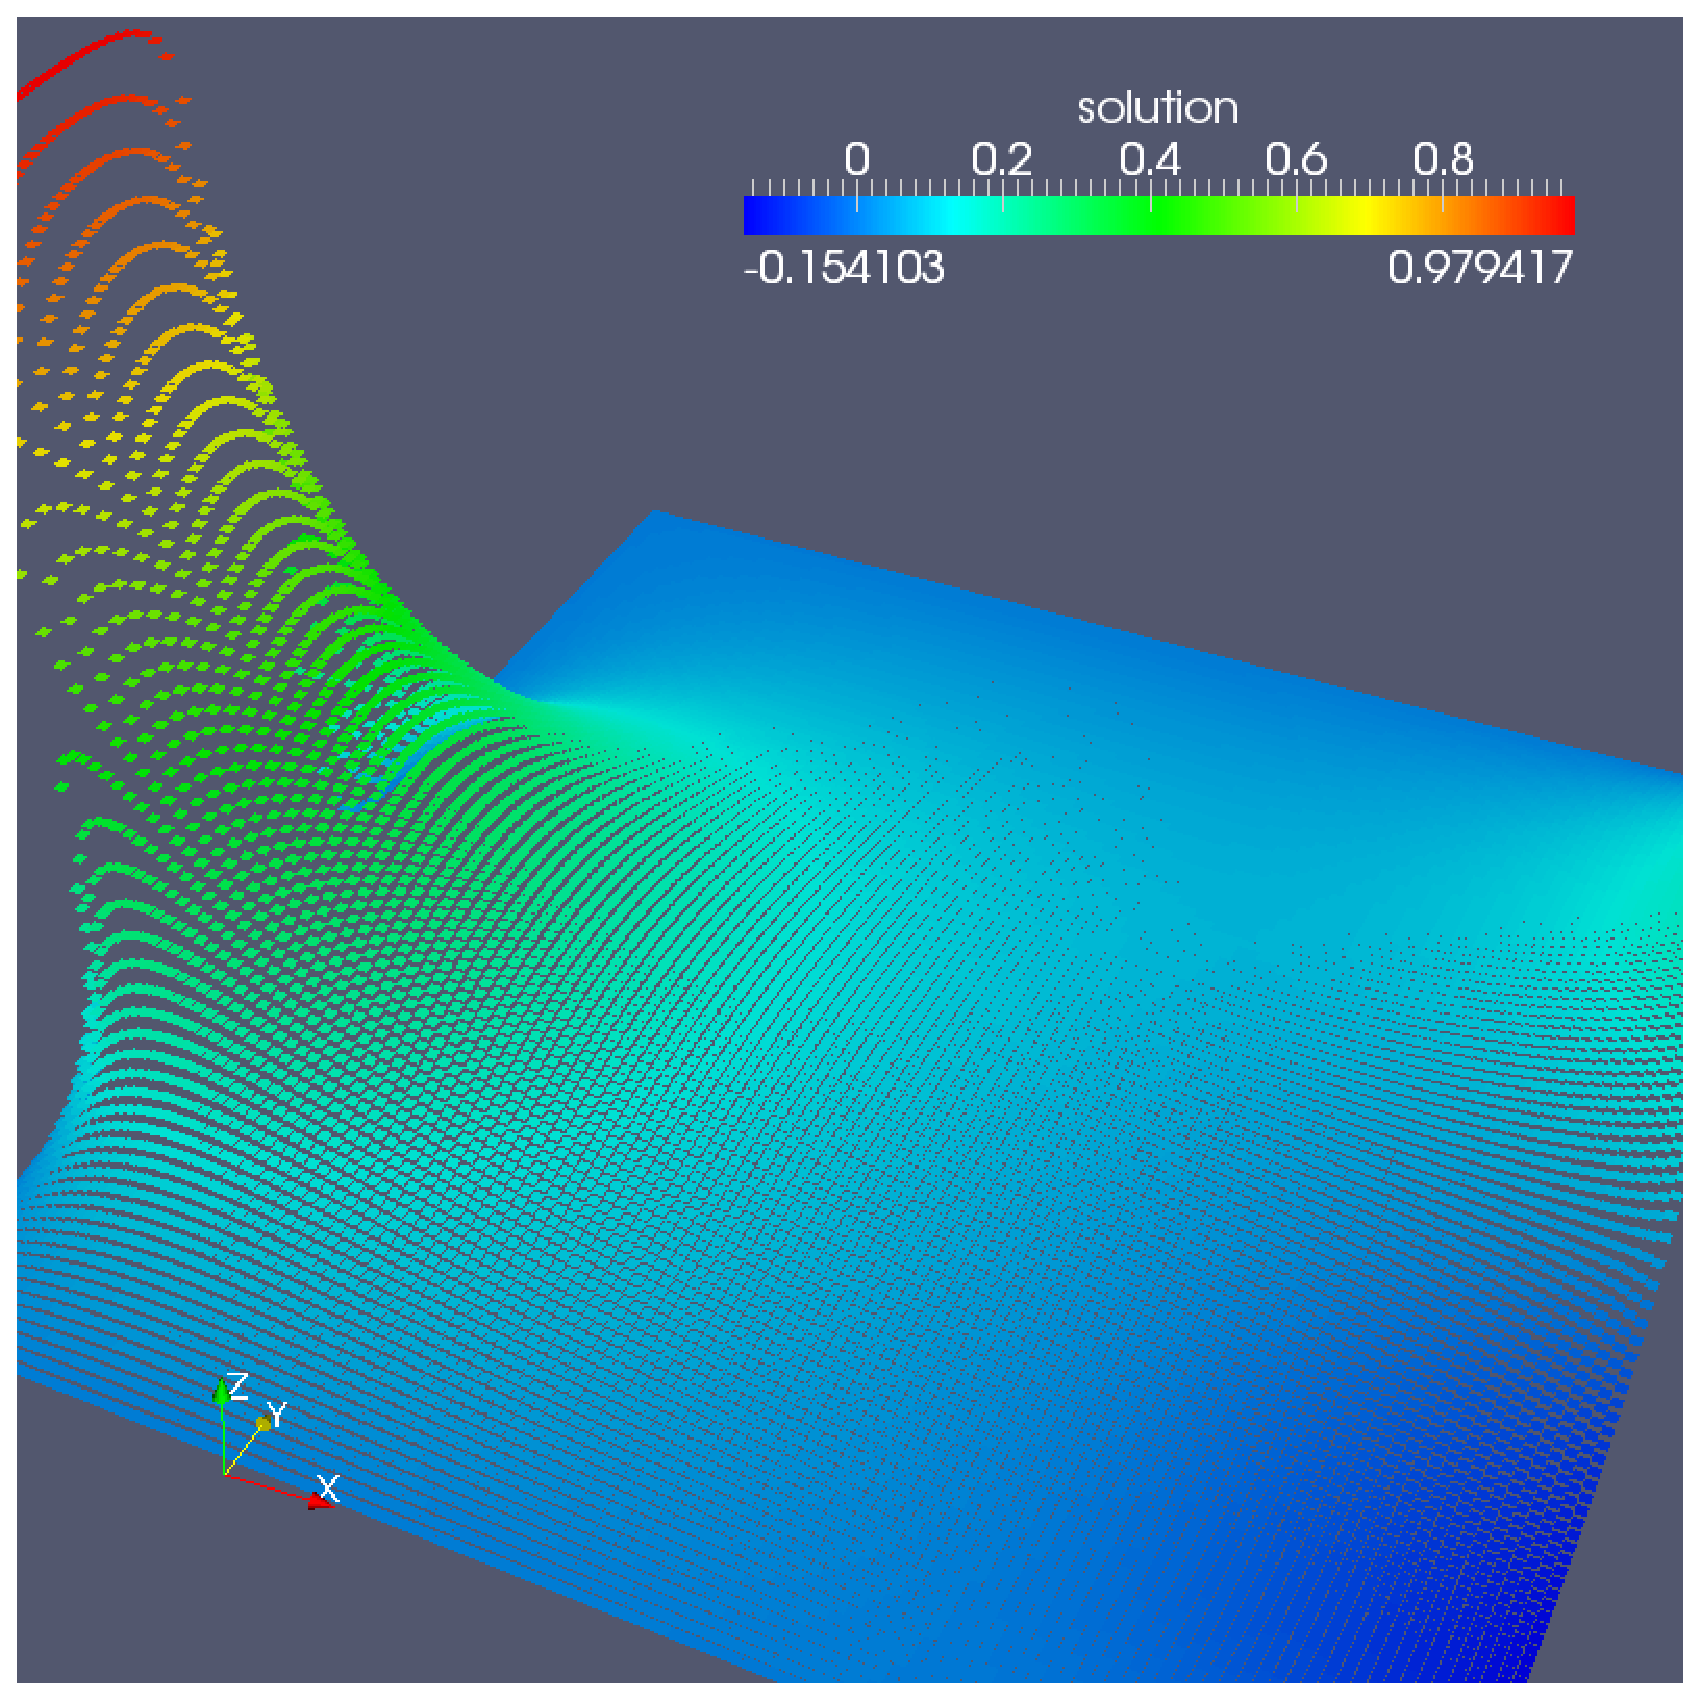
\includegraphics[width=0.48\textwidth]{./EPS/example04}
%\end{center}
%
%Conforming $Q_1$ from example 2 left and cell-centered finite volumes from example 4 right.
%\end{frame}

%-------------------------------------------------------------------
\subsection{Salome}

% Constructing Geometries
% Export von geo und unv
% Ausblick: Reader

%-------------------------------------------------------------------
\subsection{Other useful Open Source CAD-Tools}
% Uebersicht ueber andere nuetzliche CAD-Tools

\begin{frame}
  \frametitle{Overview: Other Open Source CAD-Tools}
  \begin{table}
    Table \ref{tab:CADTools} shows some other useful CAD-Tools which are able to
    export geometry or mesh files suitable for Gmsh import.
    \begin{center}
      \begin{tabular}{|c|c|c|c|c|c|c|}
        \hline
        Tool & Licence & Description & Geom & Geom & Mesh
        \\
        &  &  & Import & Export & Export
        \\
        \hline
        \hline
        Gmsh &  &  &  &  &
        \\
        \hline
        Salome & LGPL & &  &  &
        \\
        \hline
        BRLCad & GPL/BSD & &  &  &
        \\
        \hline
        GCad3D & \lstinline!.igs, .iges! & &  &  &
        \\
        \hline
        Blender & \lstinline!.geo! & CSG &  &  &
        \\
        \hline
        PythonOCC & \lstinline!.geo! & Python Wrapper for OpenCascade &  &  &
        \\
        \hline
      \end{tabular}
      \caption{Some CAD tools.}
      \label{tab:CADTools}
    \end{center}
  \end{table}
\end{frame}

\cleardoublepage
